% mnras_template.tex
%
% LaTeX template for creating an MNRAS paper
%
% v3.0 released 14 May 2015
% (version numbers match those of mnras.cls)
%
% Copyright (C) Royal Astronomical Society 2015
% Authors:
% Keith T. Smith (Royal Astronomical Society)

% Change log
%
% v3.0 May 2015
%    Renamed to match the new package name
%    Version number matches mnras.cls
%    A few minor tweaks to wording
% v1.0 September 2013
%    Beta testing only - never publicly released
%    First version: a simple (ish) template for creating an MNRAS paper

%%%%%%%%%%%%%%%%%%%%%%%%%%%%%%%%%%%%%%%%%%%%%%%%%%
% Basic setup. Most papers should leave these options alone.
\documentclass[a4paper,fleqn,usenatbib]{mnras}

% MNRAS is set in Times font. If you don't have this installed (most LaTeX
% installations will be fine) or prefer the old Computer Modern fonts, comment
% out the following line
\usepackage{newtxtext,newtxmath}
% Depending on your LaTeX fonts installation, you might get better results with one of these:
%\usepackage{mathptmx}
%\usepackage{txfonts}

% Use vector fonts, so it zooms properly in on-screen viewing software
% Don't change these lines unless you know what you are doing
\usepackage[T1]{fontenc}
\usepackage{ae,aecompl}

%%%%% AUTHORS - PLACE YOUR OWN PACKAGES HERE %%%%%

% Only include extra packages if you really need them. Common packages are:
\usepackage{graphicx}	% Including figure files
\usepackage{amsmath}	% Advanced maths commands
\usepackage{amssymb}	% Extra maths symbols
\usepackage[xindy]{glossaries}
\glsdisablehyper
\usepackage{subcaption}
\usepackage{tabularx}
\captionsetup{compatibility=false}
\usepackage[normalem]{ulem}

%%%%%%%%%%%%%%%%%%%%%%%%%%%%%%%%%%%%%%%%%%%%%%%%%%

%%%%% AUTHORS - PLACE YOUR OWN COMMANDS HERE %%%%%

% Please keep new commands to a minimum, and use \newcommand not \def to avoid
% overwriting existing commands. Example:
%\newcommand{\pcm}{\,cm$^{-2}$}	% per cm-squared

\newcommand{\GSF}[1]{\noindent\textcolor{blue}{GSF:#1}}
%comments by Marisa
\newcommand{\cM}[1]{\textcolor{magenta}{ #1 --M}}

%glossary
\newacronym{alfa}{ALFA}{Arecibo L-Band Feed Array}
\newacronym{dm}{DM}{Dispersion Measure}
\newacronym{frb}{FRB}{Fast Radio Burst}
\newacronym{fwhm}{FWHM}{Full-Width at Half-Maximum}
\newacronym{gbt}{GBT}{Greenbank Telescope}
\newacronym{if}{IF}{Intermediate Frequency}
\newacronym{igm}{IGM}{Intergalactic Medium}
\newacronym{ism}{ISM}{Interstellar Medium}
\newacronym{lo}{LO}{Local Oscillator}
\newacronym{nip}{NIP}{Non-image Processing}
\newacronym{pll}{PLL}{Phased-locked Loop}
\newacronym{rfi}{RFI}{Radio-frequency Interference}
\newacronym{rrat}{RRAT}{Rotating Radio Transient}
\newacronym{ska}{SKA}{Square Kilometre Array}
\newacronym{sefd}{SEFD}{System Equivalent Flux Density}
\newacronym{snr}{S/N}{Signal-to-Noise Ratio}
\newacronym{sps}{SPS}{Single Pulse Search}
\newacronym{tab}{TAB}{Tied-Array Beam}
\newacronym{vlbi}{VLBI}{Very-Long Baseline Interferometry}
\newacronym{xao}{XAO}{Xinjiang Astronomical Observatory}

%%%%%%%%%%%%%%%%%%%%%%%%%%%%%%%%%%%%%%%%%%%%%%%%%%

% Title of the paper, and the short title which is used in the headers.
% Keep the title short and informative.
%\title[FRB Detections and Verification Tests]{Reporting FRB Detections
%and Verification Tests}
\title[FRB Verification Criteria and Reporting]{FRB Verification Criteria and Reporting}

% Aris Karastergiou
% KJ Lee
\author[G. Foster et al.]{
Griffin Foster$^{1,2}$\thanks{E-mail: griffin.foster@physics.ox.ac.uk},
Marisa Geyer$^{3}$,
Mayuresh Surnis$^{4,5}$
\\
% List of institutions
$^{1}$University of Oxford, Sub-Department of Astrophysics, Denys Wilkinson Building, Keble Road, Oxford, OX1 3RH, United Kingdom\\
$^{2}$Department of Astronomy, University of California, Berkeley, 501 Campbell
Hall \#3411, Berkeley, CA, 94720, USA\\
$^{3}$SKA-SA, 3rd Floor, The Park, Park Road, Pinelands, South Africa\\
$^{4}$Department of Physics and Astronomy, West Virginia University, Morgantown, WV 26505, USA\\
$^{5}$Center for Gravitational Waves and Cosmology, West Virginia University, Chestnut Ridge Research Building, Morgantown,\\ WV 26505, USA\\
}

% These dates will be filled out by the publisher
\date{Accepted XXX. Received YYY; in original ZZZ}

% Enter the current year, for the copyright statements etc.
\pubyear{2018}

% Don't change these lines
\begin{document}
\label{firstpage}
\pagerange{\pageref{firstpage}--\pageref{lastpage}}
\maketitle

% TODO: sent to simon, jon, leon oostrum (apertif confidence)

% Abstract of the paper
\begin{abstract}
% What is the point of the paper?
% What is the context of the study? What background information is necessary to understand the study?
% How was the study done?
% What is the main take away message?
% What can be said about these results, and how does this affect future work?
The one-off nature of most Fast Radio Bursts (FRBs) requires extra scrutiny when
reporting such detections as astrophysical.  The prototypical FRB is a broadband
signal, appearing to occur over a frequency range wider than the receiver
bandwidth, narrow-in-time, and highly dispersed, following a $\nu^{-2}$
relation.  But, some FRBs appear band-limited, show apparent scintillation,
complex frequency-dependent structure, or multi-component pulse shapes.  In a
search for rare signals in a noisy data set, the number of false-positive
detections is based on the detection threshold and signal filters.  Such
searches should find a number of false-positive events.  We present examples of
false-positive events that occur in multiple searches, which on initial
inspection appear to be FRB-like, but are found to be due to instrumental
variations, noise, and radio frequency interference (RFI).  Differentiating
these false-positive detections from astrophysical events, requires knowledge
and tests beyond performing a thresholded single-pulse detection.  We discuss
post-detection analysis, verification tests, and data sets which should be
provided when reporting an FRB detection.
\end{abstract}

% Select between one and six entries from the list of approved keywords.
% Don't make up new ones.
\begin{keywords}
radio continuum: transients -- methods: observational
\end{keywords}

%%%%%%%%%%%%%%%%% BODY OF PAPER %%%%%%%%%%%%%%%%%%

\section{Introduction}
\label{sec:intro}

% NOTE: moved here to force the figure higher up in the text
\begin{figure*}
    \centering
    % watermark:terrestrial-frb-letter/notebooks/ALFABURST_events.ipynb
    \begin{subfigure}[t]{0.45\textwidth}
        \centering\captionsetup{width=.95\linewidth}
        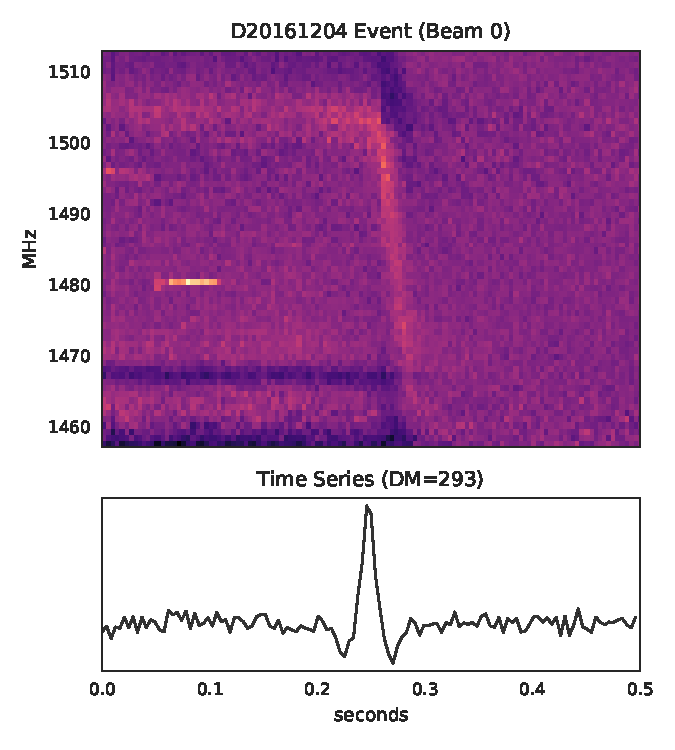
\includegraphics[width=1.0\textwidth]{figures/D20161204_buf23_Beam0.pdf}
        \caption{Detected FRB-like event in Beam 0 of ALFA. The characteristic
        dip before and after the event is due to zero-DM removal which is part
        of the ALFABURST RFI exciser. The strong, narrowband source at 1480~MHz
        around 0.1~s is due to a local RFI source.}
        \label{fig:beam0_dynamic_spec}
    \end{subfigure}
    % watermark:terrestrial-frb-letter/notebooks/ALFABURST_events.ipynb
    \begin{subfigure}[t]{0.45\textwidth}
        \centering\captionsetup{width=.95\linewidth}
        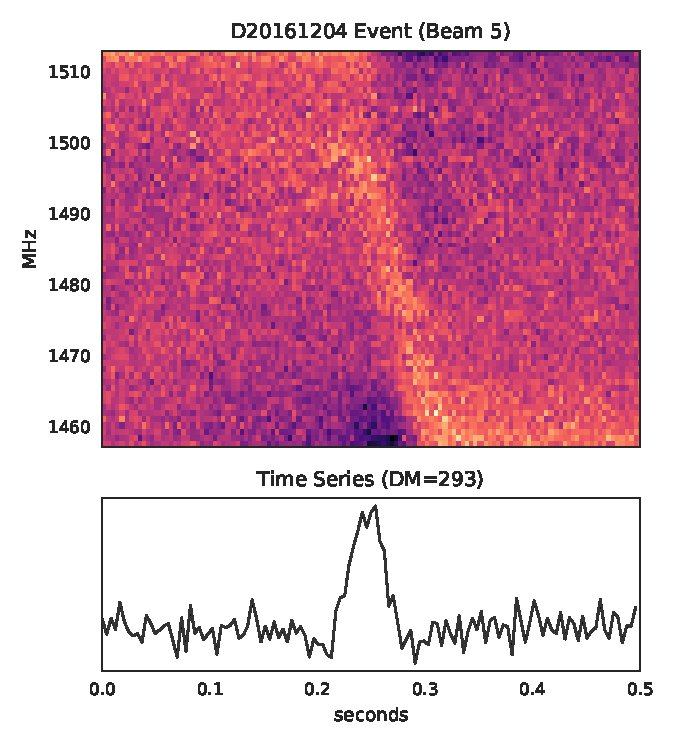
\includegraphics[width=1.0\textwidth]{figures/D20161204_buf4_Beam5.pdf}
        \caption{Detected FRB-like event in Beam 5 of ALFA. The event width
        appears wider than the Beam 0 event as the zero-DM dips are not as
        prominent.
        }
        \label{fig:beam5_dynamic_spec}
    \end{subfigure}
    \caption{
    Dynamic spectrum (top) and \gls{snr}-maximized dedispersed time series
    (bottom) of an FRB-like event that was detected simultaneously in Beam 0 and
    5 of the ALFA receiver on December 4, 2016. The dynamic spectrum has been
    bandpass normalized.
    }
    \label{fig:dynamic_spec}
\end{figure*}

The origin of \glspl{frb} continues to be a mystery since they were first
reported \citep{2007Sci...318..777L}. The \gls{dm} associated with the reported
events indicate they are occur well beyond our galaxy, possibly at cosmological
distances. They appear to be extremely bright, short duration events yet their
emission mechanism is not known.  This consensus has developed from the
reporting of detections with multiple telescopes, at different frequencies,
using different instrumentation. \glspl{frb} are difficult to detect as they
require high-gain telescopes which typically have a small beam size, such that
despite many thousands of observing hours only, a few dozen have been reported
as of this writing \citep{2016PASA...33...45P}.

The prototypical \gls{frb} is broad-band, appearing to be broader than most
receivers used in surveys. The pulse is narrow-in-time, on the order of a few
milliseconds in width, with a single component structure. The pulse is highly
dispersed, following a $\nu^{-2}$ relation and appears to be a one-off event
(only FRB121102 is known to repeat \citep{2016Natur.531..202S}).  Though, not
all reported detections appear to follow this prototypical form. Many show
complex frequency-dependent structure and are possibly band limited. The pulse
width varies due to either the emission process or propagation effects such as
scattering from the \gls{ism} and \gls{igm}.

These rare events are detected by automated GPU-accelerated software pipelines
that extensively search a broad range of \gls{dm} trials, pulse widths, and
starting times.  The de-dispersed time series is then thresholded, any
peaks above a minimum \gls{snr} are reported as potential detections. The number
of potential detections is usually overwhelming due to \gls{rfi} and system gain
variations. Initially, potential detections were reviewed manually. But, with
the amount of data acquired in recent surveys, it has become a significant time
effort to do so. Further, our understanding of the expected signal properties
has allowed the development of filters and models to select and prioritize
individual events \citep{2018MNRAS.474.3847F}.

As these sources are rare and generally appear not to repeat (except FRB121102),
there is an issue of verifiability. There is significant \gls{rfi} detectable at
all radio observatories, and there are known anthropogenic sources that appear
FRB-like \citep{2011ApJ...727...18B}.  Given the significant number of \gls{dm}
trials and high-time resolution of the spectra in a typical survey there are a
large number of false-positives which pass the automated post-processing
detection tests.  This is by design, as we would like to severely limit the
potential for false-negatives (type-II errors) in our detection pipelines by
accepting a number of false-positives (type-I errors).  But, given the large
sampling of the parameter search space it can be difficult, if not impossible to
differentiate between a true, astrophysical \gls{frb} (true-positive) and a
`terrestrial' \gls{frb} (false-positive) due to \gls{rfi}, systematics, or other
local effects. As the survey time increase the likelihood of detecting such a
false-positive will increase. To counter false detection of `terrestrial'
\glspl{frb}, verification criteria can be tested when reporting a detection.

In this paper, we present other examples of FRB-like sources which, after
further investigation, we show to be non-astrophysical. Using these and
previously reported \glspl{frb}, we develop a set of criteria to test detections
against and discuss the data, in addition to the detected dynamic spectrum, that
can be reported to provide a robust statement about an \gls{frb} detection.

\section{False-Positive FRB Detections}
\label{sec:false-pos}

During an \gls{frb} search survey there will be a significant number of
false-positive detections. The rate of these detections is set by the minimum
\gls{snr} threshold, the parameter search space, and the terrestrial environment
of the observatory. We use the term `terrestrial' to encompass multiple effects:
anthropogenic radio signal, variations in the observing system, and natural
signals from within the solar system.

Most false-positive events are filtered out with filters and classifier models.
The remaining events are commonly examined by eye as expert human knowledge
appears to be the best way to classify an detection but limitations in time do
not allow for all events to classified this way. On inspection, true
astrophysical events and terrestrial events can be difficult to differentiate
even by the expert.  These terrestrial events, indeed, should appear like
astrophysical \glspl{frb} as they have passed the detection pipeline tests. By
further investigation of the telescope state it is often possible to determine
the origin of an event. Though not always, this leads to the precarious nature
of reporting an \gls{frb} as astrophysical.  In this section we present examples
of such events which on initial inspection appear to be astrophysical, but after
further investigation prove to be terrestrial in origin.

\subsection{ALFA Terrestrial FRB}
\label{sec:D20161204}

In the two years of the initial ALFABURST survey \citep{2017ApJS..228...21C,
2018MNRAS.474.3847F}, over 200k 8.4-second data windows were recorded in which
the \gls{frb} search pipeline detected an event above the minimum \gls{snr}
detection threshold of 10.  The vast majority of these events were due to
\gls{rfi} and instrumental variations, while others were due to bright single
pulses of known pulsars.  The classifier model outputs an ordered list of events
based on the likelihood of the event being a pulse.

A narrow-in-time, broad-in-frequency, millisecond pulse was detected with the
ALFABURST system at MJD 57726.563263913 / Unix time 1480858266 (09:31:06 Arecibo
local time) in Beam 0 (the central beam) of the \gls{alfa}
receiver\footnote{http://www.naic.edu/alfa/} (Figure
\ref{fig:beam0_dynamic_spec}) which we label the D20161204 event for this
discussion. ALFABURST was processing 56~MHz of bandwidth between 1457~MHz and
1513~MHz. The \gls{snr} of this pulse is maximized when the pulse is dedispersed
with a \gls{dm} of 293~pc~cm$^{-3}$ and the 256~$\mu$s resolution is decimated
by a factor of 16 to a time resolution of 4~ms. The dedispersed time series shows
an approximately 20~ms \gls{fwhm} pulse.  The dip before and after the pulse is
due to the zero-DM filtering (i.e. the moving average is subtracted) during
pulse detection \citep{2009MNRAS.395..410E}. This is a simple way to remove a
drifting gain baseline at the cost of removing some of the overall pulse power,
particularly at low DM trials.

On initial inspection, this event looks like a promising new astrophysical
\gls{frb}. The flux density of the event can be computed with the radiometer
equation
%
$$
S = \textrm{SEFD} \frac{\textrm{S/N}}{\sqrt{D \; \Delta \tau \;
\Delta \nu}},
$$
%
using a \gls{sefd} of 3~Jy for the \gls{alfa} receiver. This results in a flux
density of $S = 66$~mJy from Beam 0, which would be a lower flux than any
previously detected \gls{frb} \citep{2016PASA...33...45P}. This flux estimate is
a lower limit, as we are assuming the source is at the centre of the beam. The
width is large for an \gls{frb} but within the range of those previously
reported.

Of the six other \gls{alfa} beams the event only appears in Beam 5 (Figure
\ref{fig:beam5_dynamic_spec}), which is adjacent to Beam 0.  This pulse lines up
with the Beam 0 event in time exactly, but the \gls{frb} was maximized
($S/N=16$) for a DM of 829~pc~cm$^{-3}$. Upon further inspection and testing
different DMs we found that this event appeared to decrease in width for lower
DM trials. There was \gls{rfi} clipping in this event which is known to
introduce a bias, resulting in a maximized \gls{snr} at a different DM trial.
We conclude the Beam 0 and Beam 5 event are the same event.

In the immediate period before and after the pulse there are no similar events
(Figure \ref{fig:dm_time}). The event appears to be isolated in time, with a
fairly compact representation in DM-space (Figure \ref{fig:dm_time_event})
similar to that of a single pulse from a high DM pulsar such as PSR B1859+03
(Figure \ref{fig:dm_time_B1859}).

\begin{figure}
    \centering
    % watermark:terrestrial-frb-letter/notebooks/ALFABURST_events.ipynb
    \begin{subfigure}[t]{0.5\textwidth}
        \centering\captionsetup{width=.95\linewidth}
        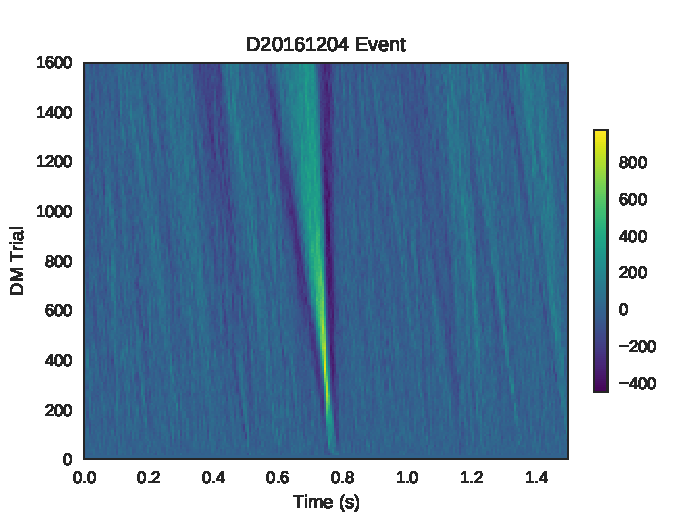
\includegraphics[width=1.0\textwidth]{figures/D20161204_dmtrials_buf23_Beam0.pdf}
        \caption{DM vs. time plot of for a 1.5~second window centred on the
        December 4th event in Beam 0. The \gls{snr} peaks at a DM of
        293~pc~cm$^{-3}$. There is a significant detection at larger DM trials
        due to the width of the pulse.
        }
        \label{fig:dm_time_event}
    \end{subfigure}
    % watermark:terrestrial-frb-letter/notebooks/ALFABURST_events.ipynb
    \begin{subfigure}[t]{0.5\textwidth}
        \centering\captionsetup{width=.95\linewidth}
        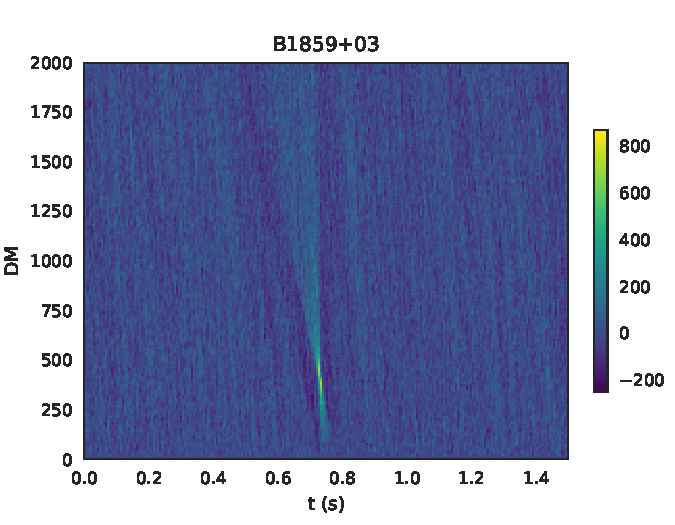
\includegraphics[width=1.0\textwidth]{figures/B1859_dmtrials.pdf}
        \caption{DM vs. time plot of a bright single pulse from B1859+03 which
        has a DM of 402~pc~cm$^{-3}$ and pulse width of 11~ms (W50).
        }
        \label{fig:dm_time_B1859}
    \end{subfigure}
    \caption{DM-space plot shows the characteristic butterfly pattern of the
    narrow-in-time, dispersed pulse detected by ALFABURST. A single pulse
    detection of B1859+03 is shown for reference.
    }
    \label{fig:dm_time}
\end{figure}

The telescope was pointed at a fixed Dec (+15:11:28.34) and drifting in RA
(event detected at RA=14:42:26.18), i.e. a fixed (alt, az) pointing during the
event. No known pulsar or RRAT with a similar DM is nearby at this pointing.

Logs provide the first indication that this event is due to a local source.  As
ALFABURST is a commensal observation survey the search pipeline regularly checks
the status of the receiver turret and \gls{if}. \gls{alfa} was logged as active and
the \gls{if} remained unchanged during this time, but the turret was in a
different position to that of where ALFA should be if it was at the secondary
focus.

The observation schedule for the morning of December 4 was project
P3080\footnote{http://www.naic.edu/vscience/schedule/tpfiles/MichillitagP3080tp.pdf}
using \gls{alfa} to perform an \gls{frb} survey of the Virgo cluster until 09:00
local time.  Followed by Project
R3037\footnote{http://www.naic.edu/vscience/schedule/tpfiles/TaylortagR3037tp.pdf},
an S-Band RADAR observation.  The event appear to have occured during a time of
no active observation, otherwise, \gls{alfa} would not have been active and in
the wrong turret position.

The average bandpass of Beam 0 and Beam 5 during the time of the event shows
that the shape and system noise appear different to what is expected during
typical observations (Figure \ref{fig:bandpass_response}).  Beam 0 and 5
bandpasses appear similar and have overlapping narrow-band RFI features that
occur during the recorded time window.  The system noise appears to be higher
during the event, which leads to smoother bandpasses than what is typical.  In
the detection pipeline the data is normalized, which removes all absolute
scaling in the process. This indicates that the \gls{sefd} is too low in our
flux calibration.  This increase in system noise is due to the change in turret
position, causing the \gls{alfa} feed to pick up reflections from other
equipment in the dome, and the dome as a warm source.  This event is most likely
due to the analogue electronics going into a non-linear state due to this
increase in system noise.

% watermark:terrestrial-frb-letter/notebooks/ALFABURST_events.ipynb
\begin{figure}
    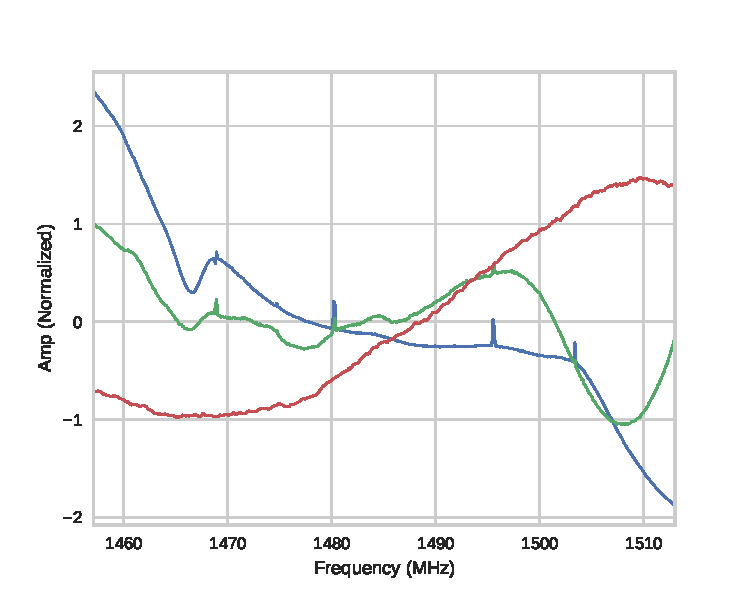
\includegraphics[width=1.0\linewidth]{figures/bandpass_response.pdf}
    \caption{Average bandpass response during the December 4, 2016 event for
    Beam 0 (green) and Beam 5 (blue). A typical bandpass (red) is plotted for
    reference. These bandpasses have been normalized in the detection pipeline.
    }
    \label{fig:bandpass_response}
\end{figure}

The theory this event is due to an analogue gain variation is further justified
by looking at data in a larger time window.  Approximately 80 seconds earlier a
window was recorded which had large structures across the band (Figure
\ref{fig:beam0_dynamic_spec_80s}). Though not as narrow in time as the event,
they appear related to the same phenomenon.  The DM$-$time plot (Figure
\ref{fig:beam0_dmtrials_80s}) shows that much of the structure would be detected
as dispersed pulses.  In particular, the structure around 4 seconds would be
detected as a wide-in-time, highly dispersed pulse.  And the structure
immediately proceeding it would be detected as a negatively dispersed pulse.  We
do not detect these as pulses because we have limited our search space to
narrow-in-time width pulses and positive \glspl{dm}.

\begin{figure*}
    \centering
    % watermark:terrestrial-frb-letter/notebooks/ALFABURST_events.ipynb
    \begin{subfigure}[t]{1.0\textwidth}
        \centering\captionsetup{width=.95\linewidth}
        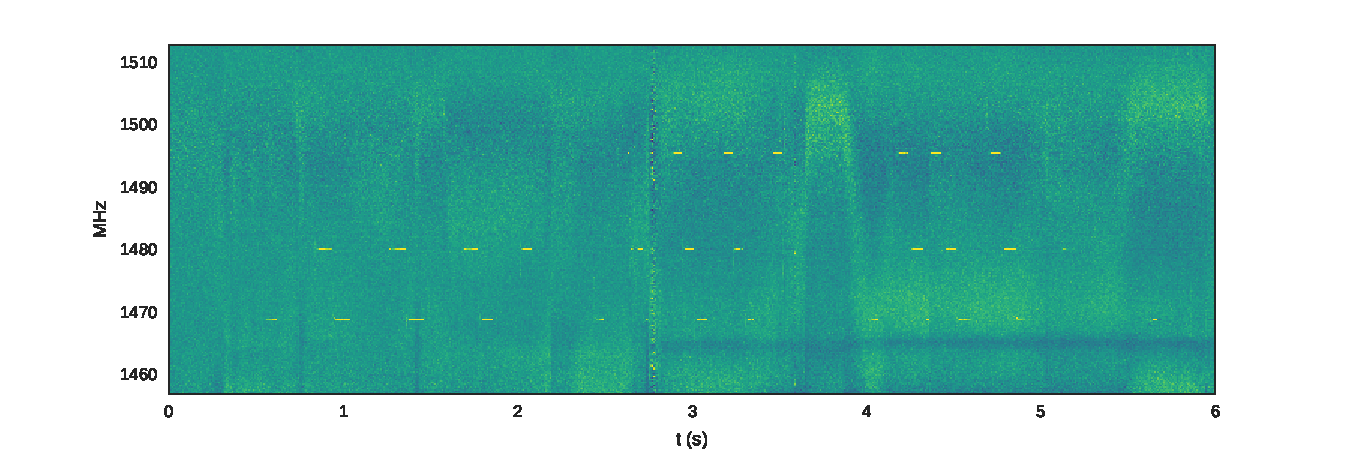
\includegraphics[width=1.0\textwidth]{figures/D20161204_spect_buf21_Beam0.pdf}
        \caption{Dynamic spectrum shows frequency evolution of the bandpass as a
        function of time with structures similar to the D20161204 event.
        }
        \label{fig:beam0_dynamic_spec_80s}
    \end{subfigure}
    % watermark:terrestrial-frb-letter/notebooks/ALFABURST_events.ipynb
    \begin{subfigure}[t]{1.0\textwidth}
        \centering\captionsetup{width=.95\linewidth}
        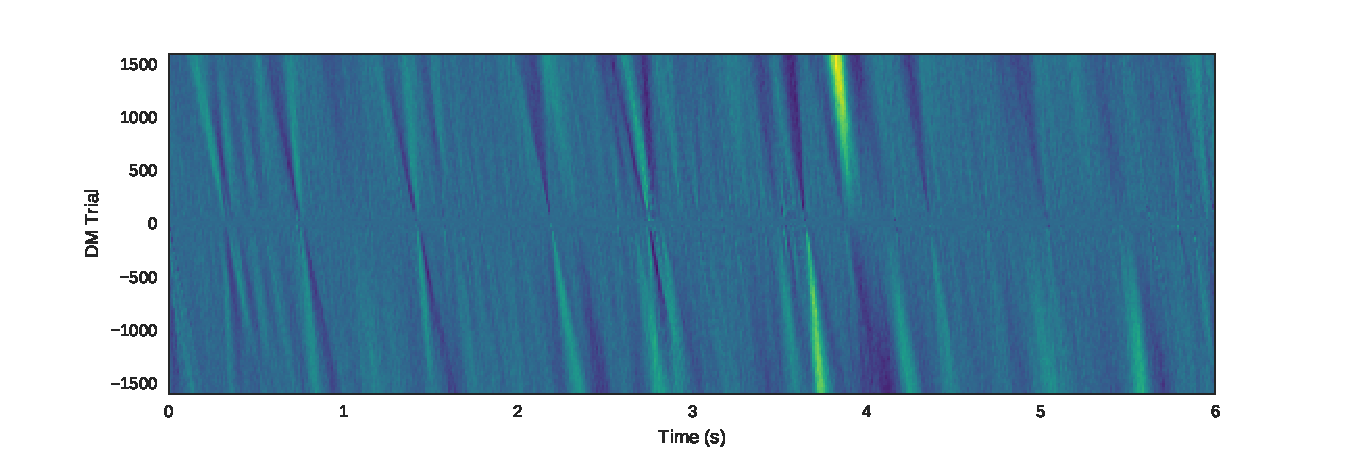
\includegraphics[width=1.0\textwidth]{figures/D20161204_dmtrials_buf21_Beam0.pdf}
        \caption{DM trials from -1600 to 1600 show that there would be both
        positive and negative pulse detections during this time window.
        }
        \label{fig:beam0_dmtrials_80s}
    \end{subfigure}
    \caption{Dynamic spectrum (top) and DM-time plot (bottom) of 6 seconds from
    beam 0 approximately 80 seconds before the D20161204 event.
    }
    \label{fig:beamo0_80s}
\end{figure*}

In isolation, and taking into account the one-off, transient nature of FRBs, the
initial Beam 0 detection reasonably appear to be astrophysical. But, after
studying the telescope state and examining data in a larger time window around
the event we can confidently classify this even as terrestrial.

\subsection{Low-S/N False-Positive Detections}
\label{sec:low_snr}

While the D20161204 event (Section \ref{sec:D20161204}) is a rare
false-positive detection based on a confluence of multiple factors, there are
other false-positive events which occur regularly.  As automated search
pipelines are set up to do an extensive search in \gls{dm} trails, pulse width,
and starting time it is reasonable to expect a large number of low-\gls{snr}
false-detections. A survey minimum \gls{snr} cut-off (usually 6-10) is set to
limit the number of these false-positives, but some of course past this minimum
cut-off threshold.

For example, on July 30, 2015 an apparently 10-$\sigma$ event with a DM of
1370~pc~cm$^{-3}$ was detected (Figure \ref{fig:D20150730}). The pulse can
barely be seen in the dynamic spectrum, but in the DM-space plot there is a
compact peak centred at a DM of 1370~pc~cm$^{-3}$ with no other similar events
apparent.  After re-analysis of the dynamic spectrum noise this event only has a
\gls{snr}$\sim$6, but was reported as a higher \gls{snr} because of the data
window size used to calculate the system noise.  Locally in time there is an
increase in system noise, leading to a reduced \gls{snr}.  From the logs it was
determined this event was due to an adjustment in the Arecibo receiver turret
position. But, this is not an uncommon event and many of these events have no
obvious explanation.

% watermark:terrestrial-frb-letter/notebooks/ALFABURST_events.ipynb
\begin{figure}
    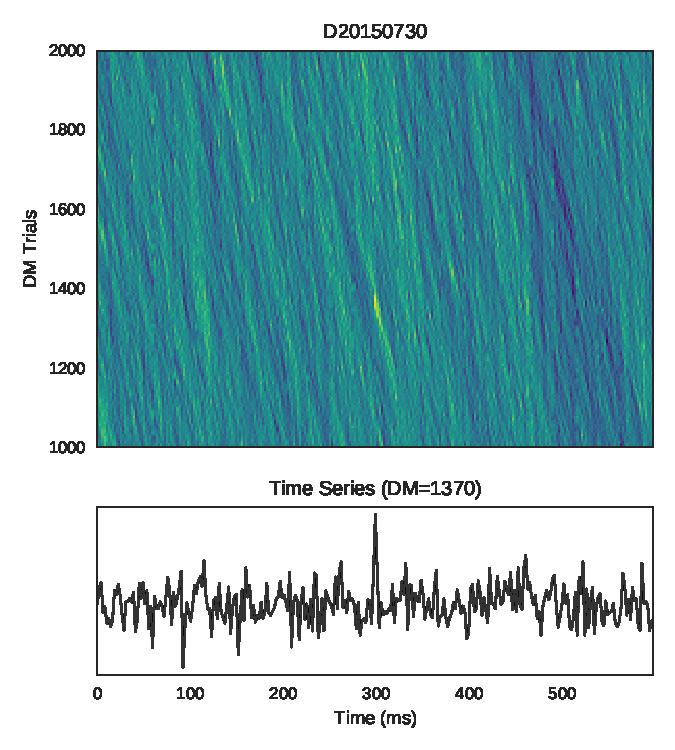
\includegraphics[width=1.0\linewidth]{figures/D20150730_buf23_Beam6_dmtrial.pdf}
    \caption{DM-space plot and time series of a high DM event with reported
    \gls{snr} above 10-$\sigma$ on July 30, 2015. After re-analysis and review
    of the telescope meta-data it was determined that this event was due to
    local system noise.
    }
    \label{fig:D20150730}
\end{figure}

These types of events prove to be difficult to validate as astrophysical or
terrestrial. If sufficient data is not recorded during a detection there will be
insufficient evidence to be confident about the event's origin. The choice of
minimum \gls{snr} is set based on the willingness of the observers to sort
through false-positive events. There are likely many low-\gls{snr} \glspl{frb}
that are labelled as false-positive events.  The reported detection of a pulse
from FRB121102 with APERTIF \citep{atel10693} had an \gls{snr}$\approx 4$. In a
blind survey across different sky positions and DM trials this would not be a
significant detection. But, the sky position and \gls{snr}-maximized DM of
FRB121102 is known, thus a lower \gls{snr} detection may be reasonable to
report.  We require a large \gls{snr} to validate a detection.  As the parameter
space (DM trials, pulse width range) and number of observations grow we expect
to see an increase in the number of high-\gls{snr}, false-positive events.

\subsection{ARTEMIS RADAR Detection}
\label{sec:LOFAR_RADAR}

ARTEMIS \citep{2015MNRAS.452.1254K} is a low-frequency \gls{frb} search survey
run on the LOFAR-UK station at Chilbolton Observatory.  The survey uses a
similar fractional bandwidth ($\sim 0.04$) to ALFABURST, but is centred at
145~MHz.  In this survey, known pulsars regularly transit the beam that are
fixed in local coordinates, and single pulses are routinely observed.  An
\gls{rfi} has been developed for this survey that successfully removes the
majority of false-positive events. Over many thousand of observing hours rare
events occasionally pass this filter.

A particularly interesting event for which the \gls{snr} was maximized at a
\gls{dm}$= 85$~pc~cm$^{-3}$ is shown in Figure \ref{fig:lofar_dynamic}. Though
this is a low DM compared to reported \glspl{frb}, this still proves to be a
relevant example as discussed later in this section.  The narrow-in-time pulse
can be seen in the dynamic spectrum at frequencies above 146 MHz, but not at
lower frequencies where it could be hidden by narrow band \gls{rfi}.  The
dedispersed time series shows a high-\gls{snr} detection of a pulse of
approximately 20~ms in width.
The beam pointing during the time of the event is not associated with any known
pulsar or RRAT around a DM$\sim$85~pc~cm$^{-3}$.

% watermark:terrestrial-frb-letter/notebooks/LOFAR_RADAR.ipynb
\begin{figure}
    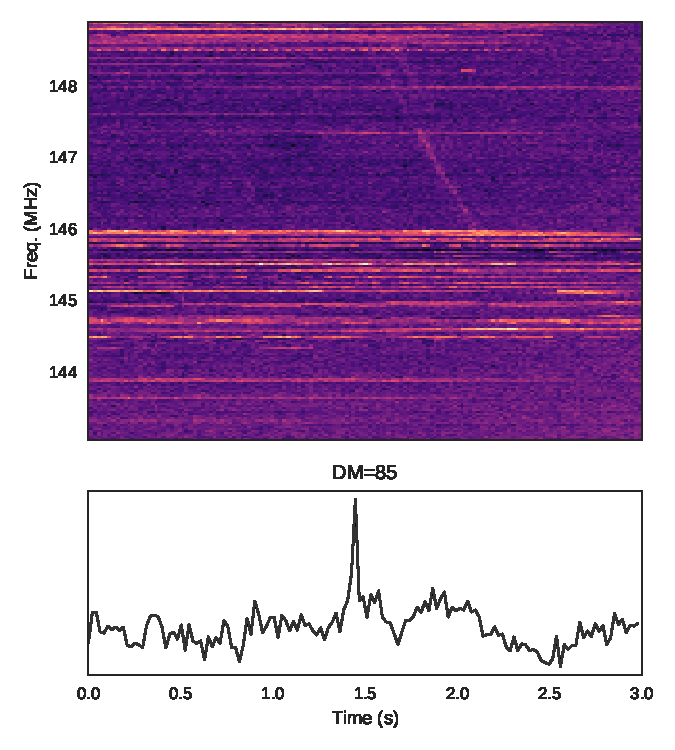
\includegraphics[width=1.0\linewidth]{figures/LOFAR_dynamic.pdf}
    \caption{A dispersed pulse detected by the automated ARTEMIS search pipeline
    at the LOFAR-UK station. The \gls{snr} is maximized when dedispersed by a DM
    of 85~pc~cm$^{-3}$. The dynamic spectrum has a time resolution of 20~ms and
    frequency resolution of 3~kHz.
    }
    \label{fig:lofar_dynamic}
\end{figure}

Plotting the event in DM-space across the ARTEMIS DM range
($0-320$~pc~cm$^{-3}$, Figure \ref{fig:lofar_dm_time}) shows a strong, compact
detection as expected of a dispersed pulse. But, the apparent limited bandwidth
of the pulse means that the pulse does not necessarily follow a $\nu^{-2}$
dispersion relation. For example, with a limited fractional bandwidth a linearly
dispersed pulse can be approximately modelled with such a relation.

% watermark:terrestrial-frb-letter/notebooks/LOFAR_RADAR.ipynb
\begin{figure}
    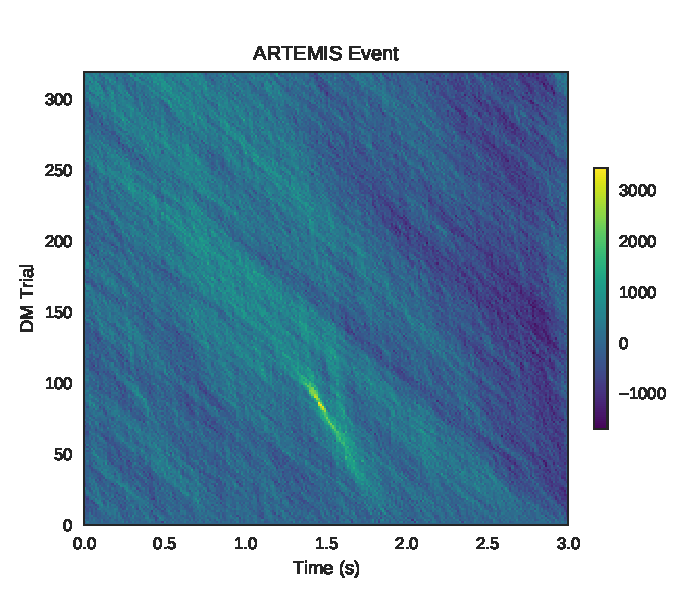
\includegraphics[width=1.0\linewidth]{figures/LOFAR_dm_time.pdf}
    \caption{DM-space plot over the DM trial range of the ARTEMIS survey. A
    strong, compact detection occurs at a DM of 85~pc~cm$^{-3}$ with no other
    apparent events during at the time.
    }
    \label{fig:lofar_dm_time}
\end{figure}

The ARTEMIS search pipeline, like most \gls{frb} search pipelines, decimates the
dynamic spectrum in time to search over a range of pulse widths. The \gls{snr}
of the event shown in Figure \ref{fig:lofar_dynamic} is maximized for a time
decimation factor of 64. With a native resolution of $327.68~\mu s$, this
results in a decimated time resolution of 20~ms. At this resolution the pulse
appears to be a continuous broadband pulse. When an event is detected in the
pipeline the undecimated dynamic spectrum is saved. Plotting at 1~ms time
resolution (Figure \ref{fig:lofar_dynamic_high}) the repeating nature of a
linear frequency-modulated signal used for pulse compression in RADAR can be
seen.

% watermark:terrestrial-frb-letter/notebooks/LOFAR_RADAR.ipynb
\begin{figure}
    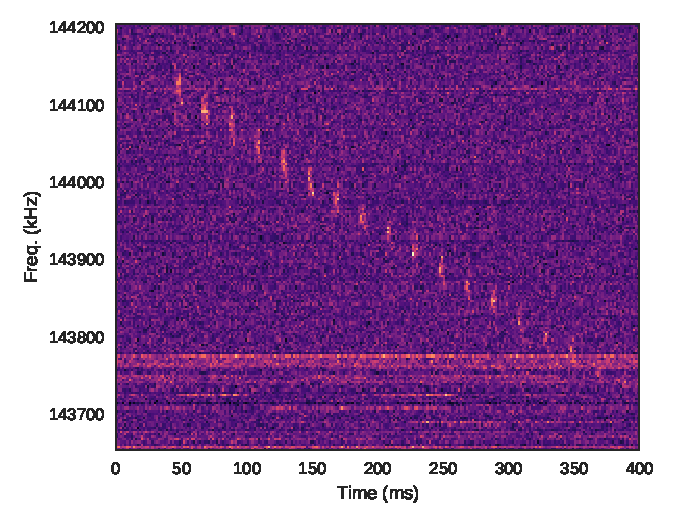
\includegraphics[width=1.0\linewidth]{figures/LOFAR_dynamic_high_res.pdf}
    \caption{A zoomed in view of the event in Figure \ref{fig:lofar_dynamic} at
    high time (1~ms) and frequency (1.5~kHz) resolution shows the distinct
    pattern of a linear frequency-modulated RADAR pulse.
    }
    \label{fig:lofar_dynamic_high}
\end{figure}

In RADAR observations, the bandwidth of the transmitter provides information on
the range and direction of a target. A narrow-band RADAR transmitter can be used
to approximate a larger bandwidth by modulating the frequency of the transmitted
pulse. The narrow-band (in frequency) pulse is stepped in frequency across a
transmission band. Between each step the pulse is not transmitted, resulting in
the gaps in time between pulses, such as in Figure \ref{fig:lofar_dynamic_high}.
An increase in the delay between the narrow-band pulses will result in a
wide-band pulse that appears more dispersed.

Linear frequency-modulation is the most typical form of chirp compression, but
non-linear methods are also used. Such a modulation technique may be the origin
of the detections in the next section.  There are a number of allocated RADAR
usages in the LOFAR observing band which could be the source of the observed
RADAR pulse \citep{ofcom2017}.  RADAR is used from UHF to C-band, covering a
wide range of frequencies at which \gls{frb} surveys operate. We could not
determine the exact origin of the RADAR pulse As RADAR is used for commercial
and military purposes, most of these signal specifications, modulations, and
source locations are proprietary.

As the RADAR signal is a dispersed pulse we expect to detect such signals with
\gls{frb} pipelines.  Verification of this event is straightforward when the
high-time and frequency resolution data is available to reveal the narrow-band,
pulsed nature of the event.

\subsection{XAO Repeating Event}
\label{sec:xao_event}

The 25-m Nanshan Telescope at \gls{xao} is currently running an FRB survey which
covers over 300~MHz at L-band, sampling at $64 \; \mu s$ resolution. On November
18, 2016 hundreds of bright, dispersed pulses were detected. The pulses varied
in \gls{snr}, but had the same \gls{snr}-maximized DM of 531.8~pc~cm$^{-3}$. The
pulses show a distinct double peak (each peak $\sim 2$~ms wide) separated by
$\sim 3$~ms (Figure \ref{fig:xao_dynamic}). The pulses are only apparent in a
portion of the band.

% watermark:/home/griffin/data/XAO/coadd_pulses.ipynb
\begin{figure}
    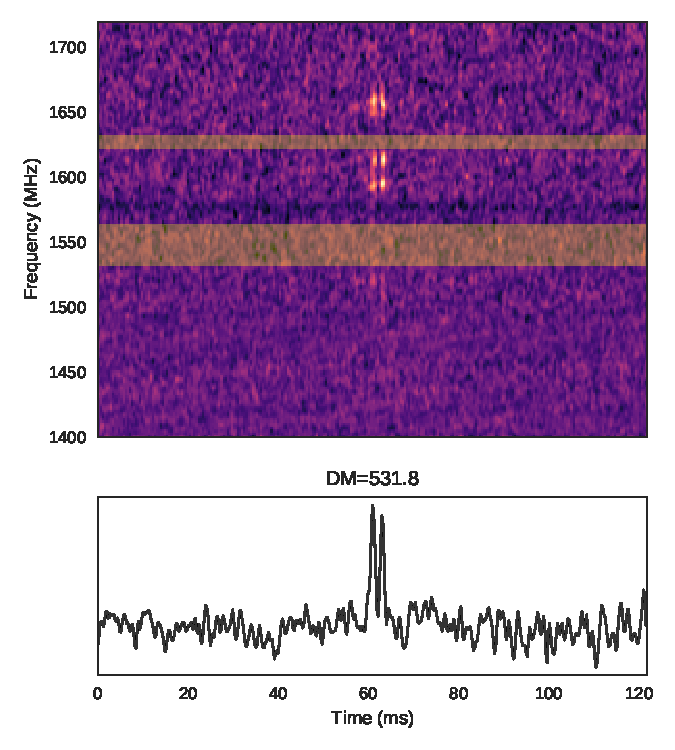
\includegraphics[width=1.0\linewidth]{figures/XAO_pulse_dynamic.pdf}
    \caption{Example of a detected pulse with the Nanshan Radio Telescope at XAO
    which is \gls{snr} maximized at a dedispersion of $531.8$~pc~cm$^{-3}$.
    Hundreds of such pulses were detected over a period of a few days. The
    orange bars represent regions that have had significant constant-in-time
    \gls{rfi} replaced by noise.
    }
    \label{fig:xao_dynamic}
\end{figure}

A periodicity search revealed a periodicity of $\sim 1.7$~s, but the residuals
were orders of magnitude higher than that of a typical pulsar periodicity
search.  Further, the pulses were seen at different pointings across the sky.
Most were detected at a low altitude pointing angle, but some were detected
close to zenith.  This rules out a pulsar, or an astronomical source in general.

Figure \ref{fig:xao_summed} shows the sum of the dedispersed (using DM
531.8~pc~cm$^{-3}$) phase-aligned pulses.  This `folded' spectrum shows an
S-shaped broadband pulse which covers most of the observing band. There is also
regular, narrow-band frequency modulation ($\sim4$~MHz) in the pulse structure.
The structure is likely due to non-linearly frequency modulation, used in
chirped RADAR systems, similar to the linear frequency-modulated signal observed
in Section \ref{sec:LOFAR_RADAR}.

% watermark:/home/griffin/data/XAO/coadd_pulses.ipynb
\begin{figure}
    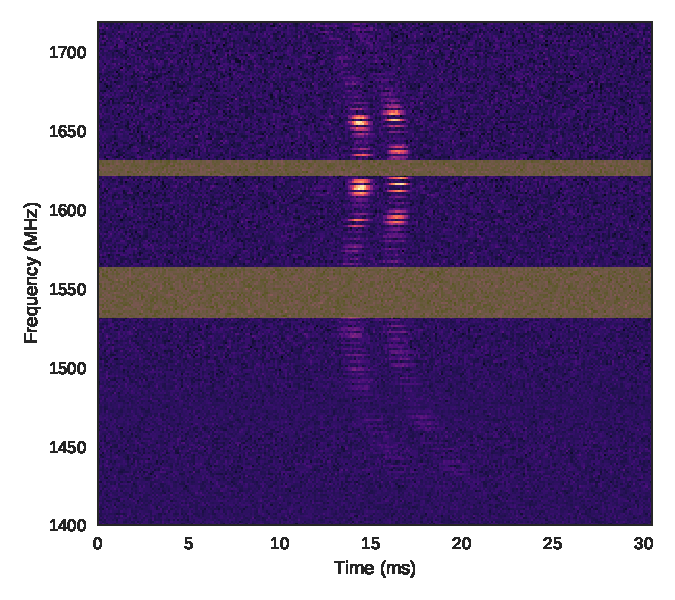
\includegraphics[width=1.0\linewidth]{figures/XAO_summed_dynamic.pdf}
    \caption{The `folded' dynamic spectrum of 182 high-\gls{snr} pulses detected
    with the Nanshan Radio Telescope.  The low-level, non-linear frequency
    modulation can be seen across the band. The orange bars represent regions
    that have had significant constant-in-time RFI \gls{rfi} replaced by noise.
    }
    \label{fig:xao_summed}
\end{figure}

A thorough search of possible local sources, such as new equipment, vehicles,
and aircraft was preformed, with no obvious candidate being found. Detection of
multiple pulses at different beam pointings indicates the source may be directly
illuminating the feed. The source is likely not due to system electronics
because of the complex frequency modulation but rather due to a local
transmitter.

The Nanshan L-band receiver is a single pixel system. It could be
that a multi-beam system such as the Parkes Multi-beam or ALFA would detection
these events in many of the beams, and the event could be classified as
terrestrial.

Had only a single pulse been detected, for example if the source was weaker, or
the telescope was only sensitive to the highest \gls{snr} event, it would be
difficult to show that the event was due to \gls{rfi}.  Multiple reported
\glspl{frb}, including the repeater FRB121102, do not cover the entire observing
band. This has been explained by various intrinsic or intermediate effects
(scintillation, plasma lenses). In the case of a single detected pulse, it would
be reasonable to report it as an astronomical \gls{frb}.

A dispersion relation parameter estimation of the individual pulses was found to
deviate from a $\nu^{-2}$ relation by $1.5 \sigma$. A dispersed astrophysical
source should always follow a cold plasma $\nu^{-2}$ relation. As shown, sources
which approximately fit this relation will still be detected with dedispersion
algorithms.

The \gls{snr}-maximized DM of the XAO events is due to the frequency structure
of the pulse, but also the receiver system.  Knowing the broadband structure of
the source, we can build a simple model to show that a non-linear modulation
scheme can produce a range of apparent \gls{snr}-maximized events depending on
the observing band compared to the pulse transmission band.

The pulse can be modelled using a logistic function which covers a bandwidth from
$\nu_{\textrm{p,0}} = 1350$~MHz to $\nu_{\textrm{p,1}} = 1750$~MHz (Figure
\ref{fig:xao_simulation_diagram}). The time duration of the pulse $\Delta
t_{\textrm{pulse}}$ is fixed such that central frequency range of the pulse has
an \gls{snr}-maximized DM of approximately 530~pc~cm$^{-3}$. The pulse is given
a width ($\Delta t_{\textrm{width}}$) by convolving the logistic function with a
3~ms wide Gaussian. The amplitude pulse is set to unity across the extent of the
band.

% figures/simulation_digram.odg
\begin{figure}
    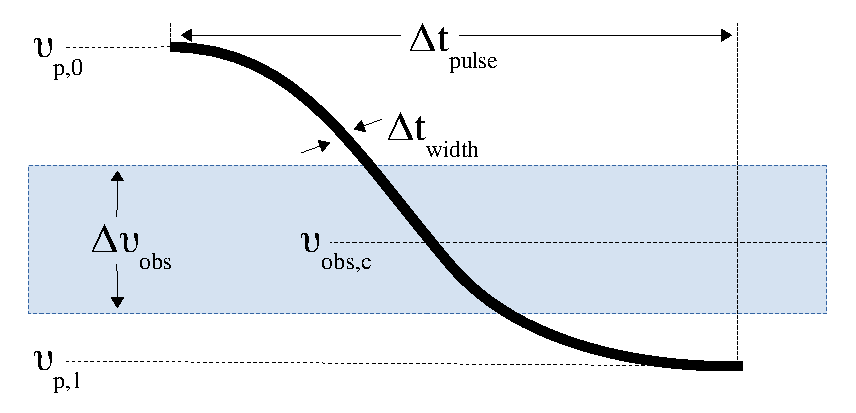
\includegraphics[width=1.0\linewidth]{figures/simulation_diagram.pdf}
    \caption{Non-linearly modulated pulse (logistic function) and receiver model
    used to simulate the response and \gls{snr}-maximized DM fit to a pulse
    similar to the one detected at XAO.
    }
    \label{fig:xao_simulation_diagram}
\end{figure}

A receiver model is used to simulate the observation. This model is
parameterized by a central observing frequency $\nu_{\textrm{obs,c}}$, bandwidth
$\Delta \nu_{\textrm{obs}}$, number of observing frequency channels
$n_{\textrm{freqs}}$, and per channel noise $\sigma_{\textrm{chan}}$. The
bandpass is modelled as a Gaussian.

% watermark:/home/griffin/data/XAO/Non-Linear-Pulse-Simulation.ipynb
\begin{figure}
    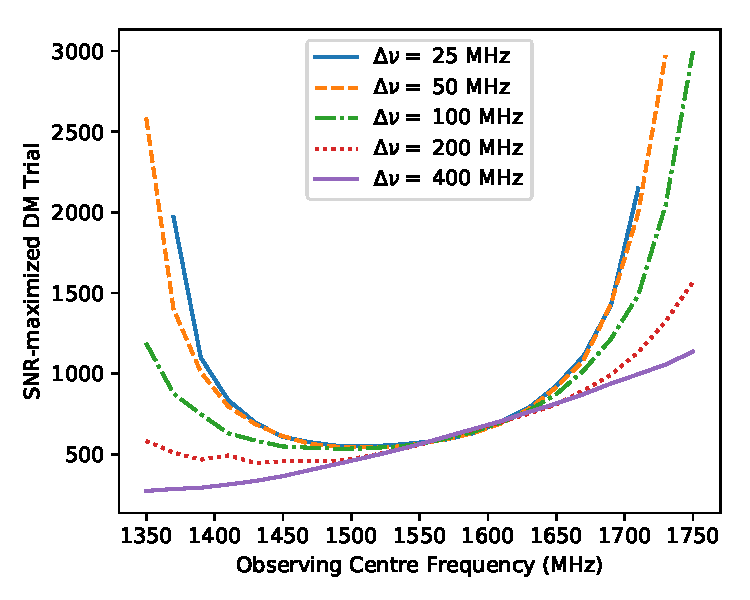
\includegraphics[width=1.0\linewidth]{figures/simulatedRADARdm.pdf}
    \caption{\gls{snr}-maximized DM trials for a simulation of the XAO
    non-linearly modulated pulse centred at 1550~MHz over a range of central
    observing frequencies, and receiver bandwidths.
    }
    \label{fig:xao_simulated_dm}
\end{figure}

Detection of the pulse is simulated across a range of central observing
frequencies and receiver bandwidths (Figure \ref{fig:xao_simulated_dm}). The
\gls{snr}-maximized DM is determined by performing a trial DM search from 0 to
4000~pc~cm$^{-3}$ in integer increments.  For all bandwidths, when the central
observing frequency is near the centre of the pulse the apparent DM of
$\sim530$~pc~cm$^{-3}$ maximizes the detection \gls{snr}. However, when the
central observing frequency is shifted relative to the pulse centre frequency a
range of \gls{snr}-maximized DM's are reported, depending on the receiver
bandwidth. This model can be used to approximate an astrophysical \gls{frb}
signal at any frequency and bandwidth for a given receiver.

Since the initial detection of the pulses in November 2016 the pulses have not
be re-detected. While the source is terrestrial in origin, these pulses present a
situation where terrestrial sources can easily be misidentified as one-off
astrophysical events. This event, along with the other events presented in this
section should present a case for developing common criteria, observing
strategies, and data recording to improve the confidence in \gls{frb}
detections.

\section{FRB Verification}
\label{sec:verify_crit}

Before reporting an \gls{frb} detection there are a set of criteria a group will
check through. This could include looking at the dynamic spectrum for \gls{rfi},
checking a DM-time space plot to see the event is compact, look at the telescope
pointing, see if the event appears in multiple beams in a multi-beam feed, etc.
There is no formal criteria, rather a set of community standards which vary
between groups and instruments. These standards are usually set in order to
compare a new detection in reference to a prototypical \gls{frb} which is broad
band, dispersed following a $\nu^{-2}$ relation in excess of the Galactic line
of sight, and narrow in pulse width such as FRB130626
\citep{2016MNRAS.460L..30C} (Figure \ref{fig:FRB130626}).

% FRB130626
% aslxlap07:/local/griffin/data/FRB/FRB130626/FRB130626.ipynb
\begin{figure}
    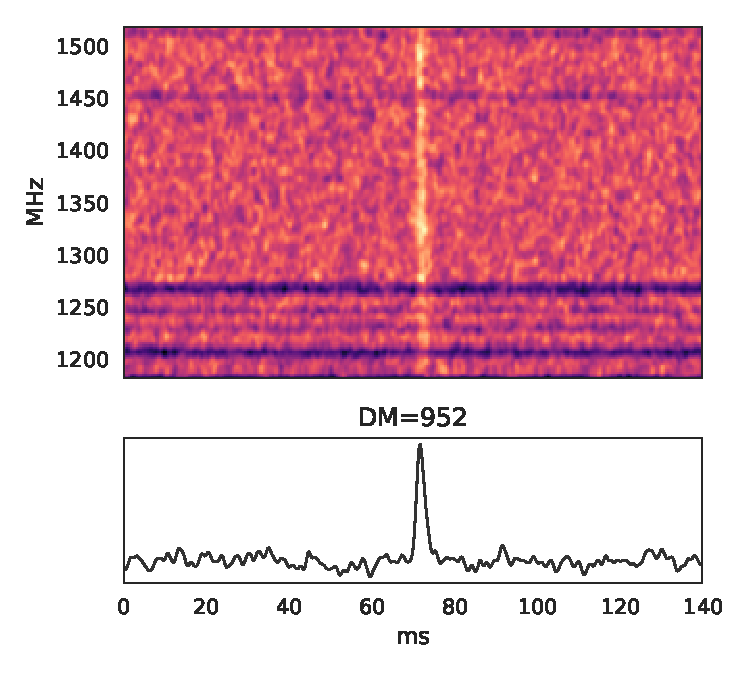
\includegraphics[width=1.0\linewidth]{figures/FRB130626.pdf}
    \caption{FRB130626 is a prototypical FRB with a broad-in-frequency,
    narrow-in-time, single component pulse at a DM=952~pc~cm$^{-3}$ well in
    excess of the Galactic DM contribution in that line of sight.
    }
    \label{fig:FRB130626}
\end{figure}

An \gls{frb} verification would not only contain criteria which compare an new
detection to a prototypical \gls{frb}, but would also contain criteria to
discount the event as terrestrial. We attempt to enumerate a set of criteria
which can be used when stating the confidence of an astrophysical \gls{frb}
detection. Of course, this will not be a complete set. As new events are
discovered, both astrophysical and terrestrial, new tests can be included. And,
as new telescopes are used for surveys a new range of tests can be designed.
This list of criteria has primarily developed for single dish surveys.  Use of
interferometric and beamformed arrays are leading to new survey and
observational modes. These arrays will provide further tests in for confidence
in a detection that single dishes can not.

\subsection{Criteria}

The verification criteria can be separated in groups relating to the detected
pulse shape and dispersion characteristics, data quality around the time of the
detected pulse, and telescope state.

\subsubsection{Pulse Shape}

%%%%%%%%%%%%%%%%%%%%%%%%%%%%%%%%%%%%%%%%%%%%%%%%%%%%%%%%%%%%%%%%%%%%%%%%%%%%%%%%
% TODO: criterion justification
% TODO: make a template notebook

\paragraph{Signal to Noise:}

What is the measured \gls{snr} of the dedispersed, and frequency-collapsed pulse?
Is this \gls{snr} above the minimum survey threshold? The actual \gls{snr} could
be different from the reported \gls{snr} as in the Section \ref{sec:low_snr}
detection because of differences in the noise statistics time-scale.

\paragraph{Implied Boresight Flux:}

What is the implied flux based on the detection \gls{snr} and telescope
sensitivity assuming the detection occurred at boresight? Is this within the
range of previously reported fluxes?
%what is the current range?
%FRB150807 128Jy

\paragraph{Pulse Width:}

What is the pulse width of the dedispersed, and frequency-collapsed pulse? Is it
within the range of previously reported widths?
%what is the current range?

\paragraph{Multi-component:}

Are there multiple components to the pulse? How many components are there? Does
this differ by changing the dedispersion DM?
%FRB130729

\paragraph{Apparently Broad-band:}

Does the pulse appear to go beyond the observing band? At both the high and low
frequency edges?
%FRB140514

\paragraph{Apparent Spectral Index:}

Is there a measurable apparent spectral index?

\paragraph{Apparently Scattered:}

Does the pulse appear to have a scattering tail? Can a scattering model be fit
to the pulse? If so, what is the scattering time scale?

\paragraph{Apparent Scintillation:}

Does the dynamic spectrum show apparent scintillation? What is the
measured characteristic scintillation bandwidth?

\paragraph{Polarization Characteristics:}

Where full Stokes parameters measured for the pulse? Does the pulse show
polarization characteristics? Can a rotation measure be fit to the pulse?

%%%%%%%%%%%%%%%%%%%%%%%%%%%%%%%%%%%%%%%%%%%%%%%%%%%%%%%%%%%%%%%%%%%%%%%%%%%%%%%%

\subsubsection{Dispersion}

\paragraph{Complex Voltage Data:}

Was complex-voltage data recorded to allow for coherent dedispersion?

\paragraph{S/N-maximized DM Fit:}

What is the \gls{snr}-maximized \gls{dm}? How does this compare to Galactic DM
model along the line of sight? Is it well in excess of the Galactic
contribution?

\paragraph{Component-optimized DM Fit:}

If there are multiple components, what is the `component-optimized' DM, how does
it differ from the \gls{snr}-maximized DM?
% FRB121102 nature

\paragraph{Dispersion Relation:}

Does the pulse follow a cold plasma $\nu^{-2}$ dispersion relation?

\paragraph{DM Space:}

In a DM space search (positive and negative DM trials) are there other
high-\gls{snr} events nearby in time to the detected pulse?

\subsubsection{Extended Timescale Observations}

\paragraph{Repeating Events:}

Does the pulse repeat at different times? Were follow-up observations performed?
Or, was a lower-\gls{snr} search performed around the detected \gls{dm} in the
survey data? If the source does repeat, what was the time scale? And, did it
occur at different telescope pointings?

\paragraph{RFI Environment:}

Was the \gls{rfi} environment drastically different during the pulse detection
compared to typical observations? What was the effective band width of the
receiver after \gls{rfi} flagging?

\subsubsection{Telescope Characteristics}

\paragraph{Telescope State:}

Was the telescope in a valid state? I.e. were the correct electronics active,
was the feed in the correct place, was other equipment active? This is a site
and telescope-dependent criterion, which requires expert knowledge in the
system in order to test this criterion with due diligence.

\paragraph{Bandpass Variation:}

Does the bandpass during the pulse appear similar to the expected bandpass seen in
typical observations?

\paragraph{Gain Stability:}

Does the gain show similar variance over a window of time around the pulse
compared to the gain variation seen in typical observations?

\paragraph{Altitude-Azimuth Pointing:}

Where was the telescope pointing in the local reference? Was it near the horizon
or known \gls{rfi} sources?

\paragraph{Multi-beam:}

Is the receiver a multi-beam system? Was the pulse detected in multiple beams?
If so, is there a difference in \gls{snr} between beams?

\paragraph{Tied-array Beam:}

Was the pulse detected with a \gls{tab} using an array of elements? If so, was
the pulse seen in individual elements? Where multiple \glspl{tab} active during
the observation? If so, was the pulse seen in multiple beams?

\paragraph{Interferometric Array:}

Was the pulse detected while baseline correlations were recorded in an
interferometric mode? Was the pulse localized within the primary beam? Is the
pulse detected on individual baselines?

\paragraph{Multi-site Observations:}

Was the pulse detected on a multi-site observation campaign? If so, was the
pulse detected at multiple sites?

\subsection{Previous Detections}

% heat map of critera for FRBs, false-positives, pulsars
% green: good evidence for astrophysical origin
% blue: neutral evidence
% yellow: unknown from reported data
% orange: evidence for terrestrial origin, (non-critical)
% red: good evidence for terrestiral origin (critical)
% gray: not valid criterion

% cases:
%   prototypical frbs
%   odd: FRB130729, FRB140514, FRB150807
%   FRB121102
%   pulsar
%   alfaburst gain
%   lofar radar
%   xao repeater

% analysis of previous detections and criteria, reporting time scales
% not all criteria can be checked or verified, but having a standard
% allows for better experiment design

%% TODO: references
%\begin{table*}
%\centering
%\begin{tabular}{ r l l r r }
%Name      & Telescope & DM (pc~cm$^{-3}$)& Width (ms) & \gls{snr}  \\
%\hline
%FRB010125 & Parkes  & $790 \pm 3$        &  9.4 	&	17   \\ 
%FRB010621 & Parkes  & $745 \pm 10$       &  7		&	16.3 \\
%FRB010724 & Parkes  & $375$              &  5		&	23   \\ 
%FRB090625 & Parkes  & $899.55 \pm 0.01$  &  1.92	&	30   \\ 
%FRB110220 & Parkes  & $944.38 \pm 0.05$  &  5.6		&	49   \\ 
%FRB110523 & GBT     & $623.3 \pm 0.06$   &  1.73	&	42   \\ 
%FRB110626 & Parkes  & $723 \pm 0.3$      &  1.4		&	11   \\ 
%FRB110703 & Parkes  & $1103.6 \pm 0.7$   &  4.3		&	16   \\ 
%FRB120127 & Parkes  & $553.3 \pm 0.3$    &  1.1		&	11   \\ 
%FRB121002 & Parkes  & $1629.18 \pm 0.02$ &  5.44	&	16   \\ 
%FRB121102 & Arecibo & $557 \pm 2$        &  3		&	14   \\ 
%FRB130626 & Parkes  & $952.4 \pm 0.1$    &  1.98	&	21   \\ 
%FRB130628 & Parkes  & $469.88 \pm 0.01$  &  0.64	&	29   \\ 
%FRB130729 & Parkes  & $861 \pm 2$        &  15.61	&	14   \\ 
%FRB131104 & Parkes  & $779 \pm 1$        &  2.08	&	30   \\ 
%FRB140514 & Parkes  & $562.7 \pm 0.6$    &  2.8		&	16   \\ 
%FRB150215 & Parkes  & $1105.6 \pm 0.8$   &  2.88	&	19   \\ 
%FRB150418 & Parkes  & $776.2 \pm 0.5$    &  0.8		&	39   \\ 
%FRB150610 & Parkes  & $1593.9 \pm 0.6$   &  2		&	18   \\ 
%FRB150807 & Parkes  & $266.5 \pm 0.1$    &  0.35	&	     \\ 
%FRB151206 & Parkes  & $1909.8 \pm 0.6$   &  3		&	10   \\ 
%FRB151230 & Parkes  & $960.4 \pm 0.5$    &  4.4		&	17   \\ 
%FRB160102 & Parkes  & $2596.1 \pm 0.3$   &  3.4		&	16   \\ 
%FRB160317 & UTMOST  & $1165 \pm 11$      &  21		&	13   \\ 
%FRB160410 & UTMOST  & $278 \pm 3$        &  4		&	13   \\ 
%FRB160608 & UTMOST  & $682 \pm 7$        &  9		&	12   \\ 
%FRB170107 & ASKAP   & $609.5 \pm 0.5$    &  2.6		&	16   \\ 
%FRB170827 & UTMOST  & $176.4$            &  0.4		&	90   \\ 
%FRB170922 & UTMOST  & $1111$             &  26		&	22   \\
%\hline
%B1859+03  & Arecibo & $402.080$          &  11      &   20   \\ % high-DM pulsar
%D20161204 & Arecibo & $293$              &  20      &   10   \\
%D20150730 & Arecibo & $1370$             &  0.5     &    6   \\
%ARTEMIS RADAR & LOFAR-UK & $85$          &  20      &        \\
%XAO Repeater & XAO  & $531.8$            &  2       &   10>  \\
%Perytons  & Parkes  & $\sim400$          &  18.5    &   10>  \\
%\end{tabular}
%\caption{Previously reported FRBs and terrestrial events discussed in this work.}
%\label{tbl:frbs}
%\end{table*}

%\subsection{FRB130729}
%
%\cite{2016MNRAS.460L..30C} reported detection of FRB130729 along with four other
%\glspl{frb} from the HTRU survey. They note that flux only appears in the lower
%half of the band, has a double peak structure, and is potentially due to
%terrestrial \gls{rfi}.  They report a \gls{dm} of 861~pc~cm$^{-3}$ for
%FRB130729, this maximizes the detection \gls{snr}, but, by using a DM of
%852~pc~cm$^{-3}$ (Figure \ref{fig:FRB130729}) the double-peak structure can be
%seen more evident. By using this lower \gls{dm} the pulse width of the two
%components can be seen to be much more narrow than the reported $\sim 16$~ms.
%The two components are separated by approximately 10~ms, with the second
%component appearing only about half as wide in bandwidth compared to the first. 
%
%% FRB130729
%% aslxlap07:/local/griffin/data/FRB/FRB130729/FRB130729.ipynb
%\begin{figure}
%    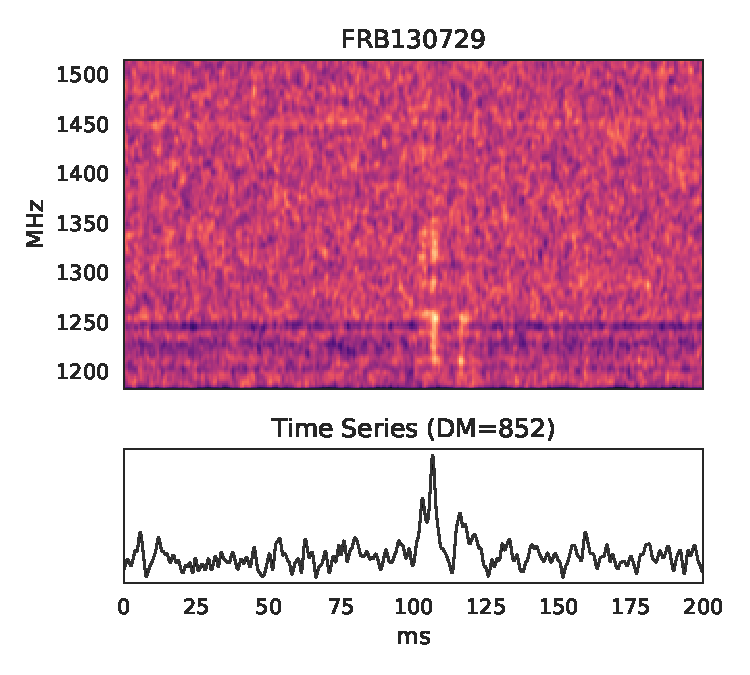
\includegraphics[width=1.0\linewidth]{figures/FRB130729.pdf}
%    \caption{FRB130729 dedispersed with a DM of 852~pc~cm$^{-3}$, this is
%    different from the \gls{snr}-maximized DM of 861~pc~cm$^{-3}$. Using this DM shows
%    that the detected FRB has two components distinct components separated by
%    approximately 10~ms. Data is presented at the native recorded resolution of
%    64~$\mu$s, 390~kHz convolved with a Gaussian smoothing filter of size
%    512~$\mu$s, 3.125~MHz.
%    }
%    \label{fig:FRB130729}
%\end{figure}

%\subsection{FRB140514}
%
%Detection of FRB140514 was reported in \citep{2015MNRAS.447..246P} and was
%reported to have significant circular polarization. But, the flux is primarily
%concentrated between 1240~MHz and 1270~MHz. This small fractional bandwidth is
%not too different from the ARTEMIS event we have reported earlier.  If this
%component is removed, for example if the observation was at a slightly different
%frequency, or smaller bandwidth, the detected \gls{snr} drops below 10.
%Further, many anthropogenic radio transmitters are circularly polarized. But,
%it could also be that there is a plasma lensing effect
%\citep{2017ApJ...842...35C} which has been used to explain the variable spectral
%index and bandwidth of FRB121102, and FRB140514 is indeed astrophysical.
%
%% FRB140514
%% aslxlap07:/local/griffin/data/FRB/FRB140514/FRB140514.ipynb
%\begin{figure}
%    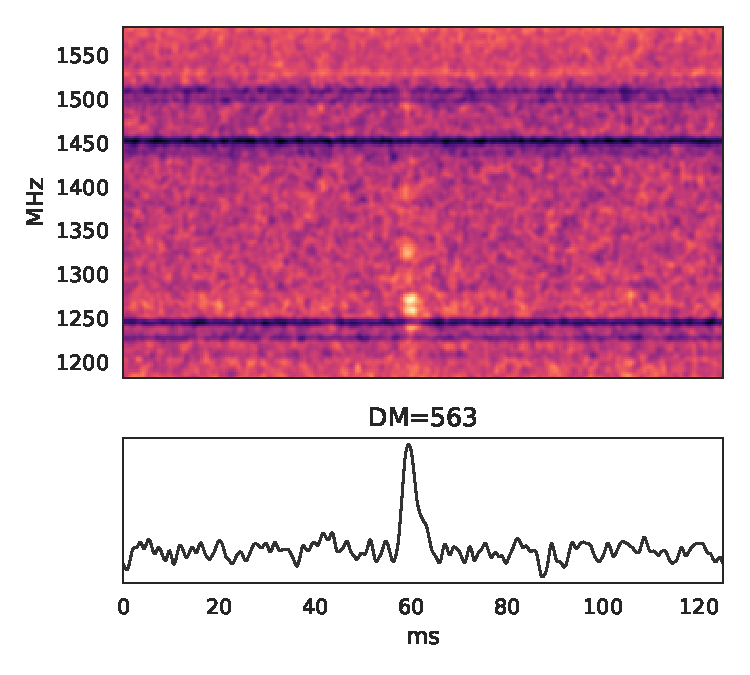
\includegraphics[width=1.0\linewidth]{figures/FRB140514.pdf}
%    \caption{The flux of FRB140514 is concentrated in a few, narrow fractional
%    bandwidth regions, primarily centred around 1260~MHz.  Data is presented at
%    the native recorded resolution of 64~$\mu$s, 390~kHz convolved with a
%    Gaussian smoothing filter of size 512~$\mu$s, 3.125~MHz.
%    }
%    \label{fig:FRB140514}
%\end{figure}

\section{Detection Reporting}

%The one-off nature of \glspl{frb} makes it essential that when reporting on a
%detection or triggering a follow-up observation that significant due-diligence
%is done in order to verify a true-positive detection as much as possible. Over the
%past decade of \gls{frb} surveys a number of techniques have been developed to
%efficiently filter for dispersed pulses. The vast majority of events are flagged
%by \gls{rfi} excisers and setting a sufficiently high minimum \gls{snr}
%threshold. This has the effect of creating potential false-negative events (i.e.
%FRBs classified as RFI), but is not useful with false-positive detections. The
%mystery and rarity of FRBs makes it difficult to differentiate astrophysical FRBs
%from local sources based on the dynamic spectrum alone. Thus, additional
%information on the observing system should be used to provide robustness to the
%detection.

\subsection{Minimum Reporting}

%At a minimum, a reasonable detection should be reported with the observed data
%made publicly available.  This allows independent verification, and can be used
%as input data sets to test pipeline development.  This is different from other
%transient detections in that astronomical pointing and observing frequency is
%sufficient to do a follow-up observation. If \glspl{frb} are indeed one-off
%event, then the detection data is the only data that will ever be available. A
%minimum reporting should include:
%
%\begin{enumerate}
%    \item Filterbank which fully encompasses the extent of the dispersed pulse.
%    \item Time and frequency resolutions, DM, and start time of detection.
%    \item Dedispered time series.
%    \item Astronomical pointing, observing frequency, and other telescope
%    observing parameters.
%    \item For a multi-beam system, filterbanks of each beam covering the extent
%    of the pulse.
%    \item A list (or guide) of software and parameters used to generate
%    detections and plots.
%\end{enumerate}
%
%These requirements are typically included in past reported \gls{frb} detections.
%The last point, a guide on which software was used is often not reported.
%Different software and data formats can have slightly different results, such as
%the reported \gls{snr} or time definition.  FRBCAT \citep{2016PASA...33...45P}
%provides a well-curated repository for this information. The atypical
%\glspl{frb} shown in Section \ref{sec:previous_frbs} are from the online data
%repositories linked in FRBCAT. Most reported \glspl{frb} detected with Parkes
%have publicly accessible data repositories which meet the reporting requirements
%stated above. As of this writing, there is no publicly available data for
%approximately a quarter of the reported \glspl{frb}. Upon publication of a
%detection, this data should be made available.
%% FRB110703: dodgy filterbank
%% FRB110523, FRB121102, FRB150807, FRB160317, FRB160410, FRB160608, FRB170107,
%% FBR170827
%% FRB150807: bright, maybe RFI

\subsection{Desirable Reporting}

%As has been shown in the previous section there are instrumentational and RFI
%sources which can produce the appearance of \glspl{frb}. Minimum reporting is
%insufficient for these non-astrophysical detections. These detection were only
%excluded with additional understanding of the telescope and observing status.
%Primarily this would be to expand the reported data in time before and after the
%detected event. Desirable reporting would include:
%
%\begin{enumerate}
%    \item Filterbank data which not only encompasses the detected pulse, but
%    includes data over a longer time span, e.g. a few minutes before and after
%    the detection. If multiple feeds were in use, data from all feeds should be
%    made available.
%    \item An expected bandpass model, and bandpass model during detection. And,
%    the measured gain variation over the observation.
%    \item Telescope observing parameters and pointing over the observation,
%    including the local (altitude, azimuth) pointing.
%    \item A DM-space plot of the detection, along with a negative DM-space
%    sampling.
%    \item A dispersion fit to the pulse.
%    \item Raw voltage or complex spectral data before power detection and
%    integration.
%\end{enumerate}
%
%Reporting of the bandpass and gain variations, along with a long time data set
%allows the state of the telescope to be understood. A deviation from normal
%operation, e.g. analogue electronics going into non-linear states, has the
%potential to produce spurious events which on a small time-scale can look
%FRB-like.
%
%A DM-space plot provides a useful diagnostic to protect against observation
%bias. An ideal detection, such as in Figure \ref{fig:dm_time_B1859}, should
%appear compact in this space, with no other detections at different trial DMs.

\subsection{False-Positive Reporting}

%During a search for anomalous signals it should be expected that there are a
%number of events reported which are false positives. Such as Perytons
%\citep{2011ApJ...727...18B} and the events reported in earlier sections. Events
%such as FRB130729 and FRB140514 are on the edge of verifiability. They do not
%fit the classic \gls{frb} model but given the available observing and system
%information, and lack of an external, anthropogenic explanation they are hard
%to discount as not being of astrophysical origin. It is necessary to report
%all of these events and to provide as much evidence as possible to explain the
%origin of such events.

% TODO: reference varying shapes of FRB121102

\section{Future Observational Methods}

%% Automated/VOevent issues:
%%Verification becomes challenging when the desire is to run the system in
%%real-time with immediate follow-up with additional telescopes.  Expert knowledge
%%in the instrument, radio signals and visual acuity were necessary to identify
%%this rare RADAR event.  Automating this process is difficult, so if we desire an
%%automated VOevent trigger, we should expect a number of false-positive triggers.
%
%Beyond detection of more \glspl{frb}, the goals of current surveys are to
%localize the source to host galaxies, and detect pulses across broader
%bandwidths across the radio spectrum.
%
%Localization requires the use of interferometric arrays. In the case of a
%compact array, a high-time resolution correlation matrix is recorded. And, in
%the case of \gls{vlbi} the raw complex voltages are recorded, which can be used
%to perform coherent dedispersion resulting in a higher resolution (time and
%frequency) dynamic spectrum of the pulses.  Related, multi-site coordinated
%observations would remove most, if not all, instrumentational and RFI sources of
%false-positive detections.
%
%Detection of \glspl{frb} at multiple frequencies not only adds to the scientific
%understanding of the sources, but also help to verify that they are
%astrophysical.  Due to historical development of receivers for pulsar searches,
%most \glspl{frb} have been detected at L-band frequencies. Though, FRB110523
%detected with the GBT and the multiple \glspl{frb} detected with UTMOST occurred
%at UHF frequencies.  Only FRB121102 has been detected above L-band.  Pulses from
%FRB121102 have been detected across a 4 GHz band (4 - 8~GHz) \citep{atel10675}.
%Such wide bands show the pulse structure goes beyond the bandwidth of known
%source of \gls{rfi} (e.g. modulated RADAR).

%\subsection{Multi-site Observations}
%
%Clear evidence for an FRB to be of astrophysical origin is the simultaneous
%detection of signal with telescopes at multiple sites. Multiple detectors, such
%as in LIGO, are essential for false-positive rejection. Coordinating telescope
%observations in logistically difficult, for example many FRB surveys run
%commensally during targetted observations, but would prove valuable in reporting
%detections.  Further, detection of an FRB at multiple bands would provide
%insight into the bandwidth characteristics of the event.
%
%Interferometric arrays provide a similar advantage to multi-site observations.
%Detections with individual recievers indicate an event is not due to systematics
%such as those in Section \ref{sec:D20161204}. And, the array can be used to
%localize the sky position. A detection could still be due to an RFI source local to
%the array, though the physical seperation of the elements and interferometric
%techniques could be used to determine if the source is in the near field.

%\subsubsection{Low-\gls{snr} Follow-up Search}
%
%Once a potential detection has been made at a given minimum \gls{snr} threshold,
%a second search should be performed focused on a DM range centred on the
%\gls{snr}-maximzed DM. This search should go to a lower minimum \gls{snr} threshold.
%Preferably this search would be over the entire observation. This test will
%serve to show whether there are additional events, similar to the XAO events,
%just below the minimum threshold, or this is a true outlier event.

%\subsubsection{Negative DM Sampling}
%
%%Our choice
%%of search space is reasonable for the type of events we wish to detect given
%%limited computing resources.
%%But, there are practical advantages to searching
%%negative \glspl{dm} and wider-in-time pulse widths. We expect astrophysical
%%pulses to have positive \glspl{dm}. But, system variation and \gls{rfi} can
%%produce signals which result in positive and negative \gls{dm} detections.  A
%%statistical measure can be computed in any time window to differentiate times of
%%significant, but low-level \gls{rfi} or system variation from actual
%%astrophysical pulses. Testing out to larger pulse widths is computationally
%%cheap as the time window is decimated, reducing the memory usage. A full
%%sampling of larger pulse widths or negative \gls{dm} trials similar to the
%%positive \gls{dm} trials is not necessary. Only a subset can be computed to
%%provide useful information on the stability of the system and the \gls{rfi}
%%environment.
%
%Current surveys typically search out to extreme \glspl{dm}, in the case of
%ALFABURST we search out to a \gls{dm} of 10000~pc~cm$^{-3}$ as the additional
%computational cost is minimum. If the \gls{dm}-redshift relation is
%approximately correct, searching to such high \glspl{dm} is sufficient to sample
%out to the very early universe. We expect an astrophysical source to be
%dispersed by a positive \gls{dm} value. As such we do not search for negatively
%dispersed pulses. But, \gls{rfi} does show up as both positive and negative
%dedispersion detections (Figure \ref{fig:beamo0_80s}). As the dedispersion
%search is no longer computationally limited it is possible to search the
%negative \gls{dm} space at low additional cost. This would be useful as a
%statistical statement about the number of positive versus negative detections to
%quantify the amount of \gls{rfi} during a detection. The full negative \gls{dm}
%space would not need to be searched, a regular sampling of the space would be
%sufficient.

%\subsubsection{Dispersion Fitting}
%
%FRB surveys, by design, search for broadband signals which follow a $\nu^{-2}$
%cold plasma dispersion relation. A distant astrophysical pulse should follow
%this relation, and any deviation from this relation is strong evidence for the
%signal being artifically generated, e.g. the XAO repeating event in Section
%\ref{sec:xao_event}. This dispersion relation can be tested on the dynamic
%spectrum of a potential FRB.
%
%The incoherent dedispersion operation aligns frequency subbands based on such a
%frequency-dependent time delay. The dynamic spectrum is averaged in frequency to
%produce a time series. Peaks above a threshold S/N are recorded as possible
%detections. But, such a detection is not necessarily maximized in S/N with at
%the cold plasma dispersion index ($\alpha = -2$). The frequency-dependent delay
%of a dispersed pulse can be modelled as
%%
%\begin{equation}
%\Delta t = A \, (\nu_1^{\alpha} - \nu_2^{\alpha}) + \Delta t_0,
%\end{equation}
%%
%where $A$ is the scaling amplitude, for $\alpha = -2$, $A = {\rm DM}$, $\nu_1$
%is the reference frequency (usually taken to be the highest frequency subband),
%and $\nu_2$ is the observing frequency of a subband.
%
%To perform the fit, the pulse signal needs to be seperated from the noise. This
%can be done with various methods. A simple method is to pick the peak flux value
%of each subband, that position corresponds to a delay and the flux value is used
%as a weight. A more advanced method would be to find the position peak after
%correlating the subband with a Gaussian pulse with a width similar to the
%detected pulse. In any method, it is useful to exclude subbands where the pulse
%is at a low S/N, and limit the maximum delay region to near the predicted
%$\nu^{-2}$ delay. The initial parameters for the fit are set to be the original
%$\nu^{-2}$ detection parameters.
%
%To produce a reasonable fit and error estimate of the dispersion index
%sufficient power needs to be present across a large enough fractional bandwidth.
%For example, system such as ALFABURST and ARTEMIS have narrow fractional
%bandwidth ($\sim 0.05$) which is insufficient to differentiate between a linear
%chirp ($\alpha = -1$) and a cold-plasma dispersed pulse. Similary, this is the
%case for a potential FRB that is only detected at significant S/N in a small
%fractional bandwidth (e.g. FRB140514).
%
%If the complex voltages are captured during a detection a better dispersion
%relation fit can be performed by doing coherent dedispersion. It is often not
%practical to store all the unaccumulated voltages during a survey. But, either
%detection triggers or short-term storage of the complex voltages be useful for
%this test which provides strong evidence for the astrophysical nature of a
%pulse.

\section{Conclusion}

%%narrative: here are some odd FRB like things, here are some odd reported
%%FRBs, it is hard to know if they are real and a ~10% false-positive rate is
%%probably fine, but bursts need to be fully reported
%
%% TODO: follow text
%%This creates a challenge of automating the triggering of follow-up with other
%%telescopes. Either there will be an excess of false-positive triggers but with a
%%short delay between detection and triggering.  Or, a non-automated, expert
%%examination of the event is required to verify, creating a delay in any
%%follow-up. Automated follow-up should be triggered when there is high confidence
%%in the likelihood of a true-positive.
%
%\glspl{frb} are unique astronomical sources from an observational point of view
%as so far no follow-up observations have been able to verify a source using a
%different telescope or observing frequency, except in the case of FRB121102
%which is known to repeat. Thus, it is necessary to provide reasonable evidence
%for an astrophysical origin when reporting a detection. 
%
%As the size and number of \gls{frb} surveys continues to increase, one expects
%an increase in the number of false-positive detections, even as rejection models
%are improved. There is a narrow line between true, astrophysical \glspl{frb} and
%false-positive events. Ancillary evidence of the telescope state and observation
%provide robust evidence for a true-positive detection. 
%
%Reporting of false-positive events, even if the source is not explained, helps
%to improve the robustness of search pipelines against systematics and \gls{rfi}.
%Reporting these events also help improve the case for \glspl{frb} being of
%astrophysical origin, just as the explanation for Perytons
%\citep{2015MNRAS.451.3933P} removed doubt about detections using Parkes.
%
%Though many previously reported \gls{frb} detections have provided sufficient
%data and telescope information, more can be provided to present a stronger case
%for the astrophysical nature of the detection. Any reported detection at the
%minimum should make the observation publicly accessible. Further, as
%observing with any radio telescope requires high expert knowledge, it is useful
%for the expert observer to include a statement of the telescope status at the
%time of a detection.
%
%Current and future surveys which search across large fractional bandwidths, and
%localize with interferometric observations will provide further evidence to
%associate an \gls{frb} detection with an astrophysical source.
%
%Jupyter notebooks and the filterbanks files are hosted on our
%public git
%repository\footnote{https://github.com/griffinfoster/terrestrial-frb-letter}.

\bibliographystyle{mnras}
\bibliography{frb-detections} 

% Don't change these lines
\bsp	% typesetting comment
\label{lastpage}
\end{document}

% End of mnras_template.tex
